
\chapter{System}
\label{chap:system}
In this chapter, the system to be control and identified is presented.
The system is a didactic manufacture system assembled from submodules fabricated
by Christiani\footnote{All images from the Christiani modules are present on its sales
  catalog, available at \url{www.christiani.de}. All rights are reserved to Christiani.}, a German
constructor specialised in Mechatronic Systems and Industry Models to
didactic ends.
This manufacture system is located in the \LCA, situated in the \UFRJ. This
system is normally used for the under-graduated studies about Industrial
Automation and control of \DESs, and also for data acquisition in some
bachelor\slash master\slash doctorate thesis, as this one.

This manufacture system is a cube assembly system, where the different cube
halves shown in \autoref{fig:cubeHalves} are put together to form cubes.
\begin{figure}[H]
  \centering
  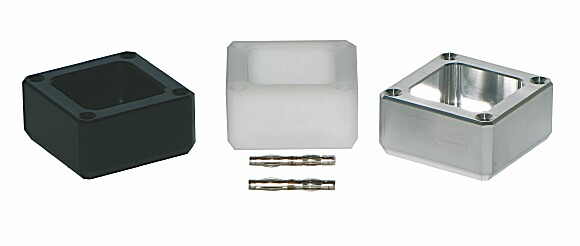
\includegraphics[width=0.55\textwidth]{maquete/pieces/workPieces.jpg}
  \caption{Cube halves.}
  \label{fig:cubeHalves}
\end{figure}

The pieces can be of two materials, metal or plastic, and the plastic ones can
be white or black.
The
permutation of cube halves needed to form a cube is selected via a type of
sorting, selecting the type of piece by material and colour. The assembled cubes
are then stored. In order to perform these tasks (sorting, handling, assembling
and stocking), 6 Units from Christiani manufacturer are used. These units can be
seen in \autoref{fig:units}.

\begin{figure}[H]
\begin{subfigure}[t]{0.325\textwidth}
  \centering
  \includegraphics[width=\textwidth]{maquete/mag/mag.jpg}
  \caption{Magazine Unit}
\end{subfigure}
\hfill
\begin{subfigure}[t]{0.325\textwidth}
  \centering
  \includegraphics[width=\textwidth]{maquete/esteira/esteira.jpg}
  \caption{Conveyor Belt.}
\end{subfigure}

\begin{subfigure}[t]{0.325\textwidth}
  \centering
  \includegraphics[width=\textwidth]{maquete/sensores/sensores.jpg}
  \caption{Sorting Unit.}
\end{subfigure}
\hfill
\begin{subfigure}[t]{0.325\textwidth}
  \centering
  \includegraphics[width=\textwidth]{maquete/braco/braco.jpg}
  \caption{Handling Unit.}
\end{subfigure}

\begin{subfigure}[t]{0.325\textwidth}
  \centering
  \includegraphics[width=\textwidth]{maquete/prensa/prensa.jpg}
  \caption{Assembly Unit.}
\end{subfigure}
\hfill
\begin{subfigure}[t]{0.325\textwidth}
  \centering
  \includegraphics[width=\textwidth]{maquete/elevador/elevador.jpg}
  \caption{Storage Unit.}
\end{subfigure}
  \caption{Units of the Manufacture System.}
  \label{fig:units}
\end{figure}

In the next sections each unit and their Inputs\slash Outputs will be detailed.

\begin{observation}
What is described in the next sections as an input of a certain module, it is
considered as an output for the controller and vice versa.  
\end{observation}

\section{Magazine Unit}
\label{sec:magazine}
The magazine is a unit with the objective to stock the cube halves to be used.
There are 2 types of magazines, one to stock pieces without connection pins (the pins shown in \autoref{fig:cubeHalves}) and another to
 stock pieces with those pins inserted, they can stack 10 and 8 pieces
 respectively. They will be denominated \verb| MAG 1| and \verb|MAG 2|.
Each magazine has a cylinder and a presence button. The cylinder serves to extract a
piece from the bottom of the stack, and the button to know if the stack is empty
or not. These cylinders have 2 inputs and 2
outputs. The inputs they are used to extend and retract the cylinders (if they
are set to $true$) and the
outputs are used to know if the cylinders are extended or retracted, the output
is equal to $true$ if the respective condition is fulfilled. These
inputs  are called in this work \verb|Extend MAG 1/2 Cylinder| and
\verb|Retract MAG 1/2 Cylinder|, and the outputs are called \verb|MAG 1/2 Cylinder Extended| and
\verb|MAG 1/2 Cylinder Retracted|. The presence button of each magazine outputs a $true$
value if the stack is empty and $false$, otherwise. Thus this presence buttons
are called in this work \verb|MAG 1/2 Empty|, their localisation on the magazine
can be seen in \autoref{fig:magazine2}. 
\begin{figure}[H]
  \centering
  \begin{tikzpicture}
    \node[anchor=south west,inner sep=0] (image) at (0,0) {
      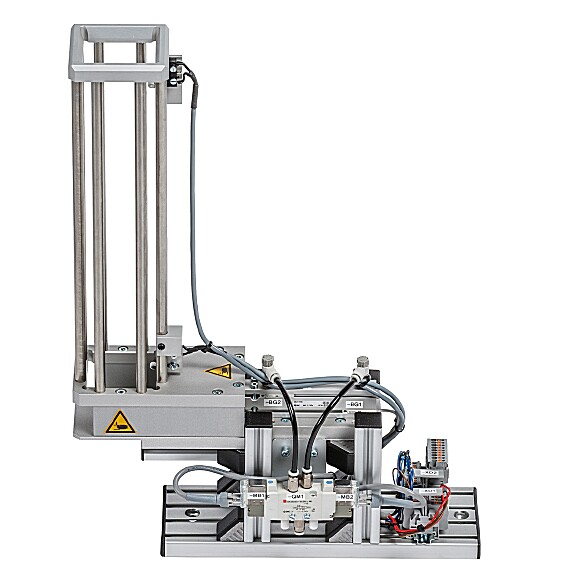
\includegraphics[width=8cm]{maquete/mag/30540_4.jpg}
    };
    % \draw[red,ultra thick,rounded corners] (0,0) rectangle (9.4,6.2);
    \begin{scope}[x={(image.south east)},y={(image.north west)}]
        % \draw[help lines,xstep=.1,ystep=.1] (0,0) grid (1,1);
        % \foreach \x in {0,1,...,9} { \node [anchor=north] at (\x/10,0) {0.\x}; }
        % \foreach \y in {0,1,...,9} { \node [anchor=east] at (0,\y/10) {0.\y}; }
      \draw[red] (0.85,0.55) node {\textbf{Cylinder}};
      \draw[<-,>=stealth,red,very thick] (0.8,0.5) -- (0.67,0.37);
      \draw[red] (0.75,0.7) node {\textbf{Presence Button}};
      \draw[red,very thick, rounded corners] (0.25,0.35) rectangle (0.35,0.45);
      \draw[<-,>=stealth,red,very thick] (0.6,0.65) -- (0.37,0.45);
      \end{scope}
  \end{tikzpicture}
  \caption{Magazine Unit.}
  \label{fig:magazine2}
\end{figure}

% only presence button
% \begin{figure}[H]
%   \centering
%   \begin{tikzpicture}
%     \node[anchor=south west,inner sep=0] (image) at (0,0) {
%       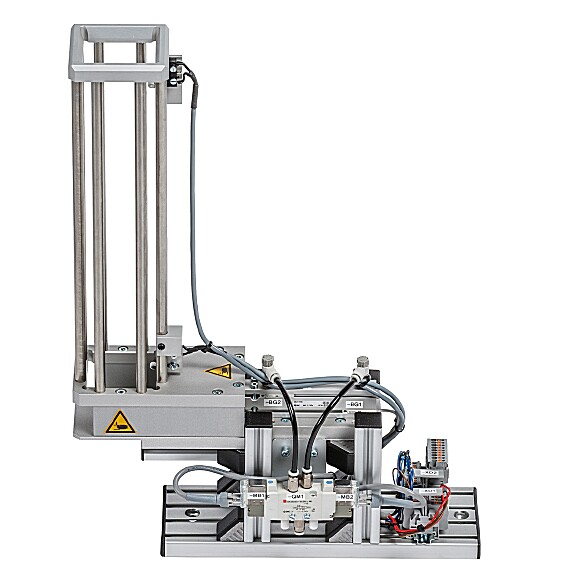
\includegraphics[width=8cm]{maquete/mag/30540_4.jpg}
%     };
%     % \draw[red,ultra thick,rounded corners] (0,0) rectangle (9.4,6.2);
%     \begin{scope}[x={(image.south east)},y={(image.north west)}]
%         % \draw[help lines,xstep=.1,ystep=.1] (0,0) grid (1,1);
%         % \foreach \x in {0,1,...,9} { \node [anchor=north] at (\x/10,0) {0.\x}; }
%         % \foreach \y in {0,1,...,9} { \node [anchor=east] at (0,\y/10) {0.\y}; }
%       \draw[red] (0.75,0.5) node {\textbf{Presence Button}};
%       \draw[red,very thick, rounded corners] (0.25,0.35) rectangle (0.35,0.45);
%       \draw[->,red,very thick] (0.5,0.5) -- (0.37,0.45);
%       \end{scope}
%   \end{tikzpicture}
%   \caption{Magazine Unit}
% \end{figure}

\section{Conveyor Belt}
\label{sec:magazine}
The conveyor belt is a unit with the objective of transporting the pieces from a
unit to another. It has 2 inputs and 1 output. The inputs are used to turn the
belt on, but each input makes it turn in a direction or the other. The output is
the generated by a presence sensor located in on extremity of the belt (see
\Autoref{fig:conveyorBelt}), it is equal to $true$ if there is a piece in front
of it and $false$ otherwise. The directions of the movement of the pieces is
denominated Forward if it is going towards the presence sensor and reverse if
not. Thus the names given to the inputs that generate this movements are
\verb|Conveyor Belt Forward| and \verb|Conveyor Belt Reverse|.
And the input is called \verb|Proximity Sensor End of Conveyor Belt|.

\begin{figure}[H]
  \centering
  \begin{tikzpicture}
    \node[anchor=south west,inner sep=0] (image) at (0,0) {
      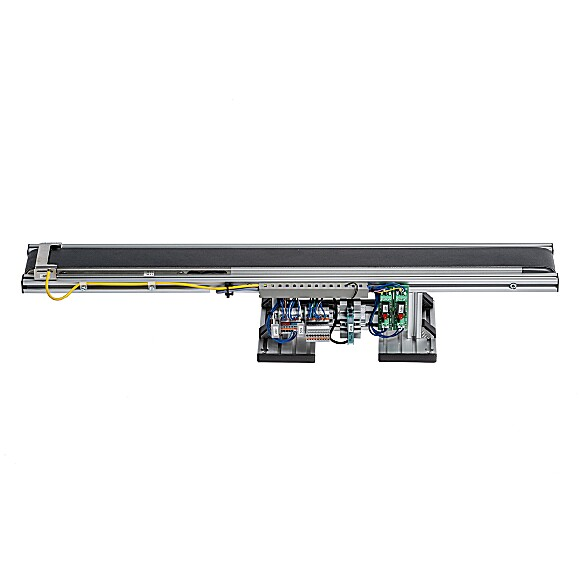
\includegraphics[trim={0 6cm 0 5cm},clip,width=8cm]{maquete/esteira/40778_3.jpg}
    };
    % \draw[red,ultra thick,rounded corners] (0,0) rectangle (9.4,6.2);
    \begin{scope}[x={(image.south east)},y={(image.north west)}]
        % \draw[help lines,xstep=.1,ystep=.1] (0,0) grid (1,1);
        % \foreach \x in {0,1,...,9} { \node [anchor=north] at (\x/10,0) {0.\x}; }
        % \foreach \y in {0,1,...,9} { \node [anchor=east] at (0,\y/10) {0.\y}; }
        \draw [->,>=stealth,red, very thick](0.9,0.75) -- ++ (-0.8,0.0);
        \draw [red] (0.5,0.85) node {Forward};
        \draw [->,>=stealth,red, very thick](0.1,0.95) -- ++ (0.8,0.0);
        \draw [red](0.5,1.05) node {Reverse};
        
        \draw [red](0.5,0.0) node {Presence Sensor};
        \draw [red,very thick,rounded corners](0.05,0.45) rectangle (0.12,0.65);
        \draw [->,>=stealth,red, very thick](0.1,0.4) -- (0.3,0.1);
      \end{scope}
  \end{tikzpicture}
  \caption{Conveyor Belt.}
  \label{fig:conveyorBelt}
\end{figure}

% no sensor
% \begin{figure}[H]
%   \centering
%   \begin{tikzpicture}
%     \node[anchor=south west,inner sep=0] (image) at (0,0) {
%       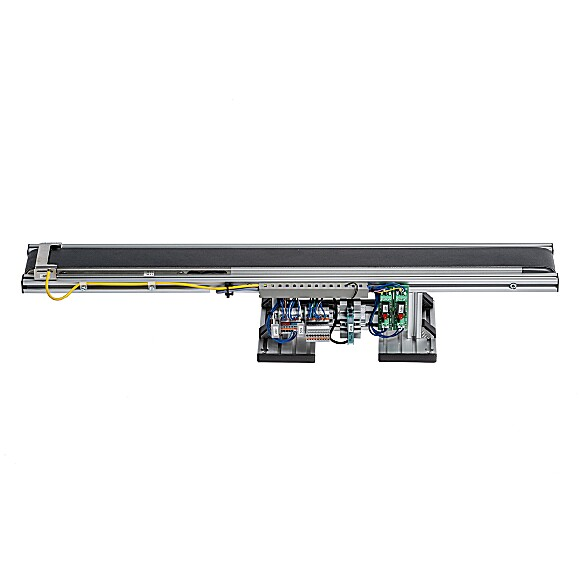
\includegraphics[trim={0 6cm 0 5cm},clip,width=8cm]{maquete/esteira/40778_3.jpg}
%     };
%     % \draw[red,ultra thick,rounded corners] (0,0) rectangle (9.4,6.2);
%     \begin{scope}[x={(image.south east)},y={(image.north west)}]
%         % \draw[help lines,xstep=.1,ystep=.1] (0,0) grid (1,1);
%         % \foreach \x in {0,1,...,9} { \node [anchor=north] at (\x/10,0) {0.\x}; }
%         % \foreach \y in {0,1,...,9} { \node [anchor=east] at (0,\y/10) {0.\y}; }
%         \draw [->,>=stealth,red, very thick](0.9,0.7) -- (0.1,0.7);
%         \draw [red] (0.5,0.8) node {Forward};
%         \draw [->,>=stealth,red, very thick](0.1,0.1) -- (0.9,0.1);
%         \draw [red](0.5,0.0) node {Reverse};
%       \end{scope}
%   \end{tikzpicture}
%   \caption{Conveyor Belt}
% \end{figure}

\section{Sorting Unit}
\label{sec:sortingUnit}
As the name says, the sorting unit serves to sort the pieces.
To understand its inputs and outputs, we will divide them in 2 parts,
identification and discharging.

The identification part uses 3 sensors to identify the type of half cube: a
distance sensor to identify the orientation of the concavity of the piece, an
optic sensor to identify the color of the plastic piece, and an inductive sensor
to identify the material of the piece. The output of the inductive sensor is
$true$ if the piece is made of metal, and $false$ if it is not, thus the given
name to this output is \verb|Metallic Sensor|. The output of the optic sensor is
equal to $true$ if the piece is reflexive (white) and $false$, otherwise
(black), thus it is named \verb|White Color Sensor|. The distance sensor outputs
an integer corresponding to the distance between the piece and the sensor, it is
named \verb|Distance Sensor|, the logic used to find the orientation of the
piece is discussed in \Autoref{chap:controlAndIdent}.
The placement of these 3 sensors can be seen in \Autoref{fig:sortIden}. 
\begin{figure}[H]
  \centering
  \begin{tikzpicture}
    \node[anchor=south west,inner sep=0] (image) at (0,0) {
      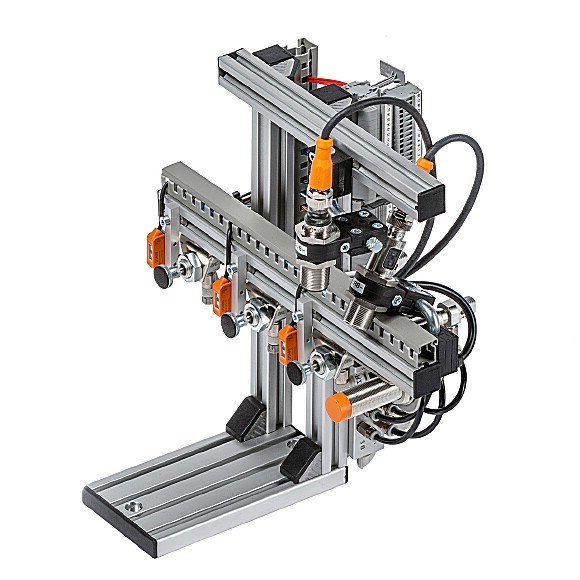
\includegraphics[trim={0 0 0 0},clip,width=8cm]{maquete/sensores/69511_2.jpg}
    };
    % \draw[red,ultra thick,rounded corners] (0,0) rectangle (9.4,6.2);

    \begin{scope}[x={(image.south east)},y={(image.north west)}]
        % \draw[help lines,xstep=.1,ystep=.1] (0,0) grid (1,1);
        % \foreach \x in {0,1,...,9} { \node [anchor=north] at (\x/10,0) {0.\x}; }
        % \foreach \y in {0,1,...,9} { \node [anchor=east] at (0,\y/10) {0.\y};  }
        \draw[red,ultra thick,rounded corners] (0.59,0.41) rectangle ++ (0.09,0.2);
        \draw[red] (0.1,0.3) node {\textbf{Optic}};
        \draw[->,>=stealth,red, very thick] (0.55,0.43) -- (0.2,0.32);
        \draw[magenta,ultra thick,rounded corners] (0.48,0.47) rectangle ++ (0.09,0.3);
        \draw[magenta] (0.1,0.8) node {\textbf{Distance}};
        \draw[->,>=stealth,magenta, very thick] (0.45,0.6) -- (0.25,0.75);
        \draw[cyan,ultra thick,rounded corners] (0.53,0.24) rectangle ++ (0.15,0.1);
        \draw[cyan] (0.6,0.05) node {\textbf{Inductive}};
        \draw[->,>=stealth,cyan, very thick] (0.6,0.2) -- (0.6,0.1);
      \end{scope}
  \end{tikzpicture}
  \caption{Sorting Unit - Identification.}
  \label{fig:sortIden}
\end{figure}

The discharging part is formed by 3 groups of inputs and outputs, denoted Left, Center and
Right, as shown in \Autoref{fig:sortDisc}. 
Each group has a cylinder and a presence sensor, and uses them to discharge pieces
depending on the logic of sorting and the identified piece by the identification
part of the sorting unit.
\begin{figure}[H]
  \centering
  \begin{tikzpicture}
    \node[anchor=south west,inner sep=0] (image) at (0,0) {
      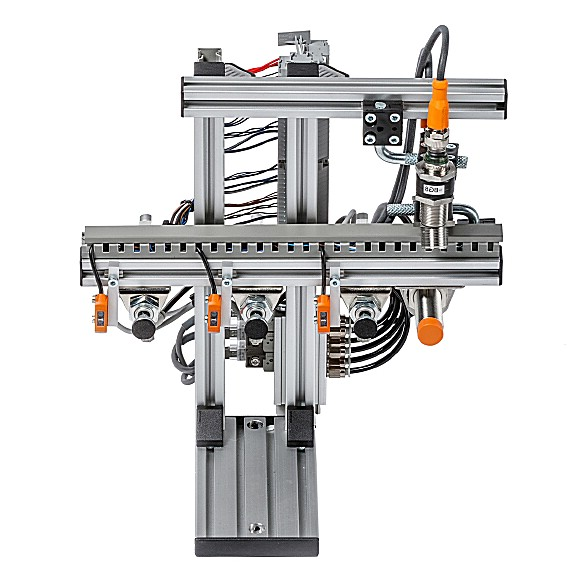
\includegraphics[trim={0 0 0 0},clip,width=8cm]{maquete/sensores/69511_3.jpg}
    };
    % \draw[red,ultra thick,rounded corners] (0,0) rectangle (9.4,6.2);

    \begin{scope}[x={(image.south east)},y={(image.north west)}]
        % \draw[help lines,xstep=.1,ystep=.1] (0,0) grid (1,1);
        % \foreach \x in {0,1,...,9} { \node [anchor=north] at (\x/10,0) {0.\x}; }
        % \foreach \y in {0,1,...,9} { \node [anchor=east] at (0,\y/10) {0.\y};  }
        \draw[red,ultra thick,rounded corners] (0.15,0.4) rectangle ++ (0.15,0.1);
        \draw[red] (0.1,0.1) node {\textbf{Left}};
        \draw[->,>=stealth,red, very thick] (0.2,0.38) -- (0.1,0.15);
        \draw[magenta,ultra thick,rounded corners] (0.35,0.4) rectangle ++ (0.15,0.1);
        \draw[magenta] (0.1,0.8) node {\textbf{Center}};
        \draw[->,>=stealth,magenta, very thick] (0.4,0.52) -- (0.2,0.75);
        \draw[cyan,ultra thick,rounded corners] (0.53,0.4) rectangle ++ (0.15,0.1);
        \draw[cyan] (0.7,0.1) node {\textbf{Right}};
        \draw[->,>=stealth,cyan, very thick] (0.65,0.38) -- (0.7,0.15);
      \end{scope}
  \end{tikzpicture}
  \caption{Sorting Unit - Discharging.}
  \label{fig:sortDisc}
\end{figure}
Differently from \verb|MAG 1/2|, each cylinder can be extended and retracted
using a single input. When the corresponding input is equal to $true$ it
extends, but when it is $false$ it is automatically retracted.
A name for each input is given depending on the group name, for
instance, to extend the left cylinder we use
\verb|Extend Left Discharge Cylinder| as input.
Each one of these cylinders has 2 outputs to determine if the cylinder is
extended or retracted, similarly the names depend on the group, e.g.:
\verb|Right Discharge Cylinder Extended| and
\verb|Right Discharge Cylinder Retracted|.
The presence sensor of each group detects if there is a piece in front of the
cylinder, and its name also depends on the group, e.g.:
\verb|Proximity Sensor Center Discharge Cylinder|.

\section{Handling Unit}
\label{sec:handlingUnit}
The handling Unit is a robotic manipulator that serves to transfer the pieces
and eventually assembled pieces, from a unit to other. By the definitions of
robotic manipulators shown in \cite{khalil2004modeling}, this manipulator has 3
\DOF{}, and it is from the type called \emph{RPP}, as
it is formed by a Revolute joint and two Prismatic joints, the latter joints
being orthogonal regarding each other.

Since the position of its
\emph{end-effector} (the end of the robotic arm) can be described using a
cylindrical coordinate system, this kind of manipulator is also called
\emph{cylindrical shoulder}. With the end of easing the understanding of the
verbs used in this work to describe the movements of the manipulator, in this
section we will use beside these verbs the cylindrical coordinate
system ($\rho,\phi,z$), where $\rho$ is the axial distance, $\phi$ is the azimuth
and $z$ is the height.
The \emph{end-effector} of this manipulator is equipped with a vacuum suction
device capable of holding the pieces. In order to control the position of the \emph{end-effector} of the manipulator, which for brevity's sake will be called
``arm'' throughout this work, there is a couple of pneumatic cylinders, whose
behaviour is similar
to the ones in the sorting unit, placed in each
prismatic joint, thus raising (increasing the height $z$) and extending (increasing the
axial distance $\rho$) the arm when they are activated respectively. The
respective inputs
of these cylinders are called \verb|Raise Arm| and \verb|Extend Arm|. Each
cylinder also has 2 outputs to identify if the are retracted or extended, the
names are given in the most mnemonic way possible, they are called
\verb|Arm Lowered|, \verb|Arm Raised|, \verb|Arm Retracted| and
\verb|Arm Extended|.

In order to rotate the revolute joint, a motor is placed
under the arm. This motor have two inputs that when activated makes the arm
rotate in one direction or the other, which will be called \CW{} and \CCW, and
the inputs that generate these kind of movements denoted
\verb|Turn Arm CW| and \verb|Turn Arm CCW|. But to identify what is considered
\CW{} and \CCW{} it is needed to impose one of those rotation direction. In this
work we imposed the \CCW{} direction as shown by the black arrow superposed to
the arm in \Autoref{fig:handlingUnit}. This same direction is considered as the
positive direction where the azimuth $\phi$ increases. The
\emph{zero position} of the arm azimuth ($\phi=0,$), is considered when the
\emph{end-effector} is diametrically opposed to the calibration pin shown in
\Autoref{fig:handlingUnit}, thus the azimuth of the arm in this figure is
$\phi=180^o$. An encoder is also present in this arm, in order to estimate the
azimuth angle, but as the angular velocity of the arm is relatively big, once
the resolution of the arm is very precise, the output of this encoder is connected to a High Speed
Counter in a \PLC, in order to correctly estimate the angle. The configuration
of the High Speed Counter can be seen in \cite{rochapereira2019automacao,antunesfloriano2019sincronizacao}.
\begin{figure}[H]
  \centering
  \begin{tikzpicture}
    \node[anchor=south west,inner sep=0] (image) at (0,0) {
      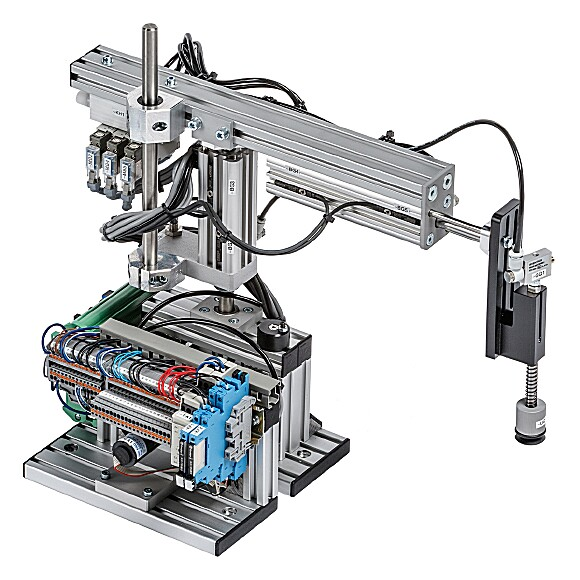
\includegraphics[trim={0 0 0 0},clip,width=8cm]{maquete/braco/69518_6.jpg}
    };
    % \draw[red,ultra thick,rounded corners] (0,0) rectangle (9.4,6.2);

    \begin{scope}[x={(image.south east)},y={(image.north west)}]
        % \draw[help lines,xstep=.1,ystep=.1] (0,0) grid (1,1);
        % \foreach \x in {0,1,...,9} { \node [anchor=north] at (\x/10,0) {0.\x}; }
        % \foreach \y in {0,1,...,9} { \node [anchor=east] at (0,\y/10) {0.\y};  }
        % \draw [fill,white,fill opacity=0.4,draw=none] (0.1,0.8) rectangle  (0.4,0.96);
        \draw [red,rounded corners, very thick] (0.43,0.4) rectangle  (0.5,0.45);
        \draw [->,>=stealth,red, very thick] (0.51,0.384) -- (0.7,0.1);
        \draw [red] (0.7,0.04) node {Calibration Pin};
        \begin{scope}[red, scale=0.1]
          \draw[black, thick] (3.5,10) arc (0:180:1 and 0.3);
        \end{scope}
        \draw[->,>=stealth,red, very thick] (0.255,0.8) -- (0.255,1.07);
        \begin{scope}[red, scale=0.1]
          \draw[black,->,>=stealth,thick] (1.5,10) arc (180:350:1 and 0.3);
        \end{scope}
      \end{scope}
  \end{tikzpicture}
  \caption{Handling Unit.}
  \label{fig:handlingUnit}
\end{figure}


\section{Assembly Unit}
\label{sec:assemblyUnit}
The assembly unit serves to mount two pieces, resulting in a fully assembled cube

\begin{figure}[H]
  \centering
  \begin{tikzpicture}
    \node[anchor=south west,inner sep=0] (image) at (0,0) {
      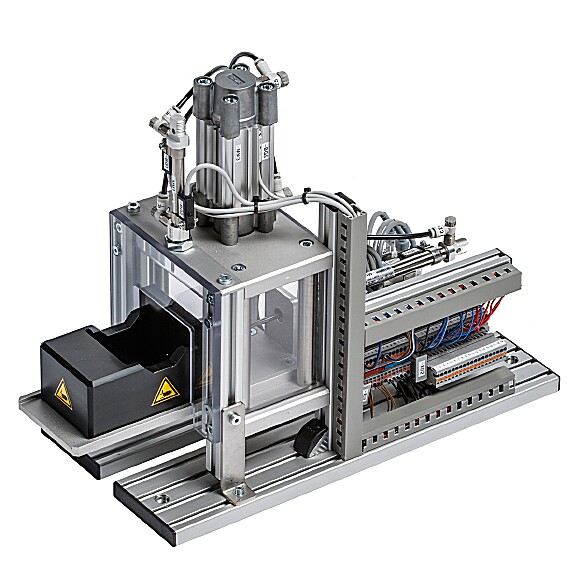
\includegraphics[width=8cm]{maquete/prensa/69514_5.jpg}
    };
    % \draw[red,ultra thick,rounded corners] (0,0) rectangle (9.4,6.2);
    \begin{scope}[x={(image.south east)},y={(image.north west)}]
        % \draw[help lines,xstep=.1,ystep=.1] (0,0) grid (1,1);
        % \foreach \x in {0,1,...,9} { \node [anchor=north] at (\x/10,0) {0.\x}; }
        % \foreach \y in {0,1,...,9} { \node [anchor=east] at (0,\y/10) {0.\y}; }
      % \draw[red] (1,0.5) node {\textbf{Right}};
      % \draw[red] (0,0.5) node {\textbf{Left}};
      % \draw[red] (0.5,1) node {\textbf{Top}};
      % \draw[red] (0.5,0) node {\textbf{Bottom}};
      \end{scope}
  \end{tikzpicture}
  \caption{Assembly Unit.}
\end{figure}

\section{Storage Unit}
\label{sec:storageUnit}
\begin{figure}[H]
  \centering
  \begin{tikzpicture}
    \node[anchor=south west,inner sep=0] (image) at (0,0) {
      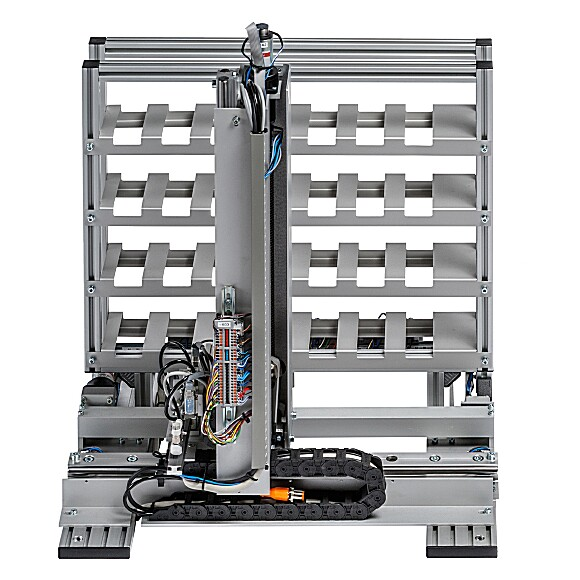
\includegraphics[width=8cm]{maquete/elevador/69523_3.jpg}
    };
    % \draw[red,ultra thick,rounded corners] (0,0) rectangle (9.4,6.2);
    \begin{scope}[x={(image.south east)},y={(image.north west)}]
        % \draw[help lines,xstep=.1,ystep=.1] (0,0) grid (1,1);
        % \foreach \x in {0,1,...,9} { \node [anchor=north] at (\x/10,0) {0.\x}; }
        % \foreach \y in {0,1,...,9} { \node [anchor=east] at (0,\y/10) {0.\y}; }
      \draw[red] (1,0.5) node {\textbf{Right}};
      \draw[red] (0,0.5) node {\textbf{Left}};
      \draw[red] (0.5,1) node {\textbf{Top}};
      \draw[red] (0.5,0) node {\textbf{Bottom}};
      \end{scope}
  \end{tikzpicture}
  \caption{Storage Unit.}
\end{figure}


%%% Local Variables:
%%% mode: latex
%%% TeX-master: "../monografia"
%%% End:
